%%%%%%%%%%%%%%%%%%%%%%%%%%%%%%%%%%%%%%%%%%%%%%%%%%%%
%												   %
%	ESCOLA   									   %
%												   %
%	Abril 2015  								   %
%												   %
%	Angela Cardoso, Rui Costa e Ricardo Lopes	   %
%   											   %	
%%%%%%%%%%%%%%%%%%%%%%%%%%%%%%%%%%%%%%%%%%%%%%%%%%%%

\documentclass[12pt,a4paper,reqno]{report}
\linespread{1.5}

\usepackage{amsfonts,amsmath,amssymb,indentfirst,mathrsfs,amscd}
\usepackage[mathscr]{eucal}
\usepackage[active]{srcltx} %inverse search
\usepackage{tensor}
\usepackage[utf8x]{inputenc}
\usepackage[portuges]{babel}
\usepackage[T1]{fontenc}
\usepackage{tikz}
\usepackage{graphicx}
\usepackage[numbers,square, comma, sort&compress]{natbib}
\numberwithin{figure}{section}
\numberwithin{equation}{section}
\usepackage{scalefnt}
\usepackage[top=2.5cm, bottom=2.5cm, left=2.5cm, right=2.5cm]{geometry}
\usepackage{comment} 
\usepackage{listings}
%\usepackage{tweaklist}
%\renewcommand{\itemhook}{\setlength{\topsep}{0pt}%
%	\setlength{\itemsep}{0pt}}
%\renewcommand{\enumhook}{\setlength{\topsep}{0pt}%
%	\setlength{\itemsep}{0pt}}
%\usepackage[colorlinks]{hyperref}
\usepackage{MnSymbol}
%\usepackage[pdfpagelabels,pagebackref,hypertexnames=true,plainpages=false,naturalnames]{hyperref}
\usepackage[naturalnames]{hyperref}
\usepackage{enumitem}
\usepackage{titling}
\newcommand{\subtitle}[1]{%
  \posttitle{%
    \par\end{center}
    \begin{center}\large#1\end{center}
    \vskip0.5em}%
}
\newcommand{\HRule}{\rule{\linewidth}{0.5mm}}

\usepackage[official]{eurosym}

\def\Cpp{C\raisebox{0.5ex}{\tiny\textbf{++}}}

\makeatletter
\def\@makechapterhead#1{%
  %%%%\vspace*{50\p@}% %%% removed!
  {\parindent \z@ \raggedright \normalfont
    \ifnum \c@secnumdepth >\m@ne
        \huge\bfseries \@chapapp\space \thechapter
        \par\nobreak
        \vskip 20\p@
    \fi
    \interlinepenalty\@M
    \Huge \bfseries #1\par\nobreak
    \vskip 40\p@
  }}
\def\@makeschapterhead#1{%
  %%%%%\vspace*{50\p@}% %%% removed!
  {\parindent \z@ \raggedright
    \normalfont
    \interlinepenalty\@M
    \Huge \bfseries  #1\par\nobreak
    \vskip 40\p@
  }}
\makeatother


\begin{document}



\begin{titlepage}
\begin{center}
 
\vspace*{3cm}

{\Large Bases de Dados}\\[1.5cm]

% Title
{\Huge \bfseries Escola Secundária \\[2cm]}

% Author
{\large Ângela Cardoso, Rui Costa e Ricardo Lopes}\\[2cm]

\includegraphics[width=10cm]{feup_logo.jpg}\\[2cm]


% Bottom of the page
{\large \today}

\end{center}
\end{titlepage}

\tableofcontents

%%%%%%%%%%%%%%
% INTRODUCAO %
%%%%%%%%%%%%%%
\chapter{Introdução}

No âmbito da unidade curricular Bases de Dados, do Mestrado Integrado em Engenharia Informática e Computação, decidimos modelar e implementar uma base de dados para gestão de uma escola secundária.

O sistema deve conter informação sobre alunos, docentes, encarregados de educação, disciplinas, turmas e áreas, permitindo a adição de novos elementos, assim como a consulta dos elementos previamente adicionados e das relações existentes entre eles.

Ao longo deste documento, além do modelo UML, considerado na versão anterior, descrevem-se o modelo relacional e a implementação em SQL que desenvolvemos para a referida base de dados. Tal como na primeira parte do trabalho, voltamos a expor as várias restrições consideradas, o tipo de situações que estão enquadradas neste modelo e aquelas que estão fora do âmbito da solução que propomos. Além disso, descrevemos as várias alterações que foram feitas relativamente à abordagem inicial.

%%%%%%%%%%%%%
% DESCRICAO %
%%%%%%%%%%%%%
\chapter{Descrição do Contexto}

Numa escola secundária há 3 grupos de pessoas fundamentais: os professores, os alunos e os encarregados de educação. Cada um destes grupos tem um papel distinto, com o objetivo comum de formar os alunos no âmbito das respetivas áreas escolhidas. Além destas pessoas, numa escola também podemos encontrar funcionários e diretores. No entanto, como veremos mais adiante, estes não são contemplados no modelo que construímos.

Além de algumas tarefas de estilo mais administrativo, como reuniões ou elaboração de relatórios, as principais responsabilidades dos professores são dar aulas e avaliar os alunos. Um professor que seja diretor de turma, tem ainda que reunir com os encarregados de educação dos alunos dessa turma, consoante as necessidades do aluno.

Os alunos têm como principais tarefas a frequência das aulas, o estudo fora destas e a realização das diversas provas de avaliação.

O encarregado de educação deve acompanhar o aluno nos seus estudos e reunir com o diretor de turma, para ajudar a optimizar o aproveitamento do aluno.

Os alunos estão organizados em turmas, consoante o ano que frequentam e a área dos seus estudos. Para cada turma há um professor responsável (o diretor de turma), um conjunto de disciplinas e um professor responsável por cada disciplina.

A escola providencia várias áreas de formação, consoante o ramo e o tipo de curso. Por exemplo, no ramo científico poderá haver áreas de carácter geral e de caráter tecnológico ou mesmo profissional. Para cada área de formação existe um professor que coordena essa área.

Um ano letivo é constituído por um ou mais períodos de avaliação. Atualmente, o ano letivo está dividido em 3 períodos, mas é possível que isso seja alterado no futuro. Em cada período os alunos são avaliados nas disciplinas que frequentam obtendo uma classificação que fica registada.

%%%%%%%%%%%%%
% DESCRICAO %
%%%%%%%%%%%%%
\chapter{Descrição da Solução Implementada}

No modelo desenvolvido, consideramos as seguintes classes principais:
\begin{itemize}
\item \textbf{Pessoa} - superclasse que contém a informação comum aos docentes, alunos e encarregados de educação, como o número de identificação na escola, o nome, a morada, a data de nascimento, etc;
\item \textbf{Docente} - tem atributos próprios, como o ano de admissão e as qualificações;
\item \textbf{Aluno} - tal como o docente, tem um ano de entrada na escola, tendo ainda um campo de observações, como por exemplo uma suspensão ou uma condição médica que seja do interesse da escola, e os campos derivados média, nota máxima e numero de disciplinas realizadas, cujo cálculo é atualizado automaticamente consoante o aluno vai completando as disciplinas;
\item \textbf{Encarregado\_Educação} - tem um horário preferencial para ser contactado pela escola, sendo esse contacto normalmente efetuado pelo diretor de turma de um dos alunos pelo qual é responsável;
\item \textbf{Área} - contém informação sobre o tipo de curso, nomeadamente, se se trata de um curso de carácter geral, tecnológico ou profissional, assim como o ramo a que pertence;
\item \textbf{Turma} - é identificada por um número e pelo ano escolar a que pertence, além disso está associada a um ano letivo específico;
\item \textbf{Disciplina} - possui um código de identificação da escola, assim como o nome e a descrição;
\item \textbf{Ano\_Letivo} - tem uma data de início, uma data de fim e uma designação, sendo constituído por vários períodos letivos;
\item \textbf{Período} - é identificado por um número, contendo ainda informação sobre as datas em que inicia e termina.
\end{itemize}

Abstraímos também os conceitos de \textbf{Código\_Postal} e \textbf{Localidade}. Além disso, temos outras classes ``secundárias'', que descreveremos mais adiante. Estas surgiram inicialmente como classes de associação, mas para que fosse possível manter histórico passaram a classes.

Em cada instante, para qualquer par turma e disciplina, existe um único professor associado. No entanto, este professor poderá ser substituído, por motivos de doença, por exemplo. Além disso, um dado professor pode estar apto a lecionar outras disciplinas além destas, estando essa informação contida na base de dados da escola. Há ainda uma relação entre cada turma e um docente específico: o diretor de turma. Uma dada turma tem um e um só diretor, que à partida será responsável pela turma durante todo o ano letivo. No entanto, em situações excepcionais, poderá ser necessária a substituição do diretor de turma, sendo isso contemplado no modelo que desenhamos.

Os alunos são classificados a todas as disciplinas que frequentam consoante o período do ano letivo. Tal como foi mencionado acima, com a adição de classificações são recalculadas a média e a nota máxima do aluno. As disciplinas frequentadas por um dado aluno são determinadas consoante a turma em que ele está inserido. Sendo que a turma, por sua vez, depende do ano escolar e da área de formação dos seus alunos.

À semelhança daquilo que acontece com os diretores de turma, cada área possui um único coordenador em cada momento. No entanto, esse coordenador poderá variar ao longo do tempo. Um dado docente não é coordenador de mais do que uma área ao mesmo tempo.

Os encarregados de educação e os diretores de turma podem marcar reuniões por iniciativa de qualquer um deles, ficando registadas a data, a hora e a sala da reunião. Excepcionalmente, um encarregado de educação poderá reunir com outro professor do aluno pelo qual é responsável, ficando essa reunião registada da mesma forma. Cada aluno possui um único encarregado de educação (que pode ser responsável por vários alunos), sendo registada a relação de parentesco do encarregado com o aluno. Em alguns casos essa relação poderá não ser familiar, no entanto é sempre usada a palavra parentesco, ainda que no sentido lato.

Consideramos que é possível uma mesma pessoa ser simultaneamente docente da escola e encarregado de educação. Além disso, embora apenas em casos muitos especiais, um determinado aluno pode ser também encarregado de educação (de si próprio ou de outro aluno), nomeadamente se esse aluno for maior de idade ou tiver sido emancipado.

No modelo que desenhamos, não são contemplados os horários das várias aulas. Sendo assim, não é possível determinar o horário de um determinado aluno ou de um professor. Também não é incluída qualquer informação sobre os funcionários da escola, sobre os seus diretores ou sobre eventuais enfermeiros ou psicólogos. Numa versão mais alargada, poderiam e deveriam ser consideradas estas classes. Também seria interessante considerar informação mais detalhada sobre o percurso do aluno na escola, como por exemplo alterações significativas na sua vida pessoal, registos de faltas, visitas à enfermagem ou ao gabinete de psicologia, testes psicotécnicos que tenha efetuado, projetos e grupos extracurriculares em que tenha estado envolvido, etc.

%%%%%%%%%%%%
% DIAGRAMA %
%%%%%%%%%%%%
\chapter{Modelo Conceptual}

\begin{center}

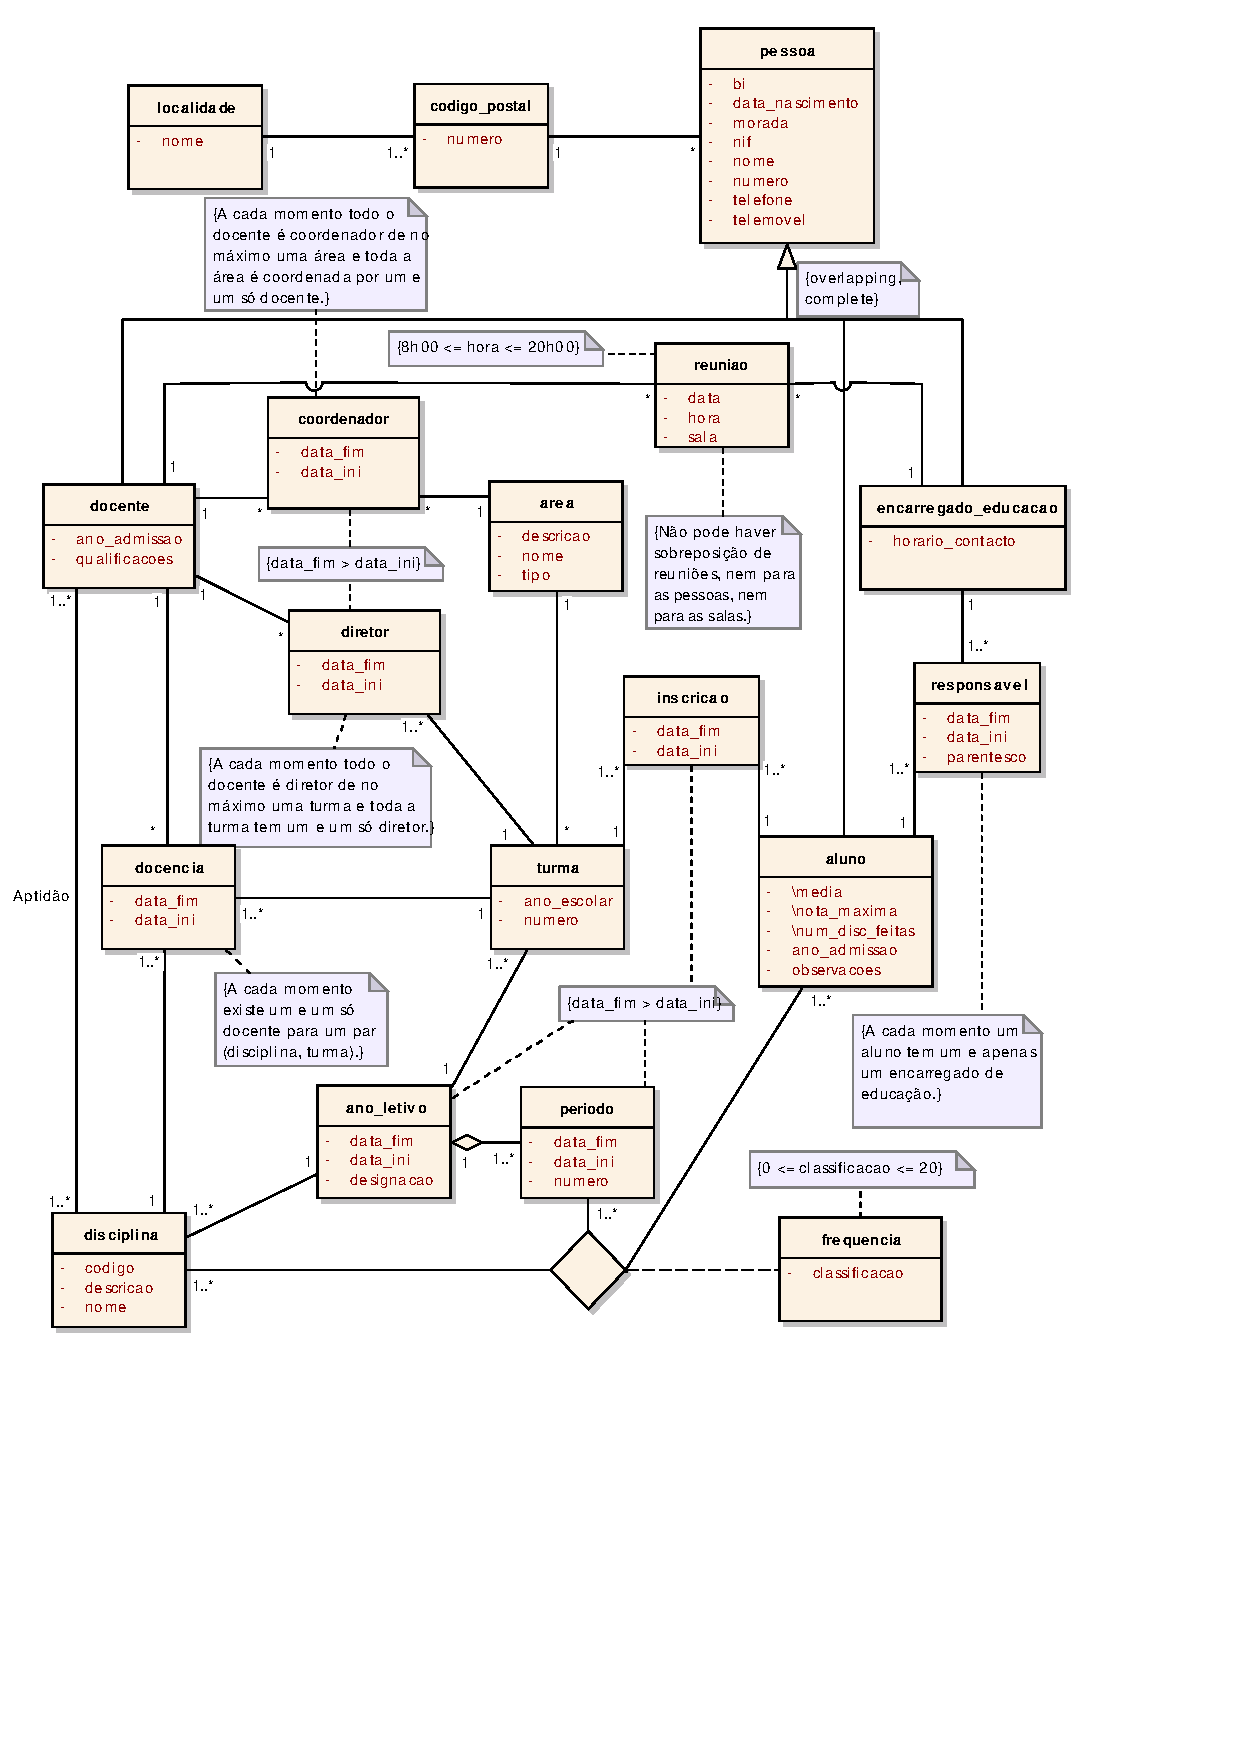
\includegraphics[width=16cm]{conceptual3.jpg}

\end{center}

%%%%%%%%%%
% MODELO %
%%%%%%%%%%
\chapter{Modelo Relacional}

\begin{itemize}

\item \textbf{localidade} (\underline{id\_localidade}, nome)

\item \textbf{codigo\_postal} (\underline {id\_cod\_postal}, numero, id\_localidade $\rightarrow$ localidade)

\item \textbf{pessoa} (\underline{id\_pessoa}, numero, nome, bi, nif, morada, data\_nasc, telefone, telemovel, id\_cod\_postal $\rightarrow$ codigo\_postal)

\item \textbf{docente} (\underline{id\_docente} $\rightarrow$ pessoa, ano\_admissao, qualificacoes)

\item \textbf{aluno} (\underline{id\_aluno} $\rightarrow$ pessoa, ano\_admissao, observacoes, media, max\_nota, num\_disc\_feitas)

\item \textbf{encarregado} (\underline{id\_encarregado} $\rightarrow$ pessoa, horario\_contacto)

\item \textbf{area} (\underline{id\_area}, nome, descricao, tipo)

\item \textbf{coordenador} (\underline{id\_coordenador}, id\_docente $\rightarrow$ docente, id\_area $\rightarrow$ area, data\_ini, data\_fim)

\item \textbf{turma} (\underline{id\_turma}, numero, ano\_escolar, id\_area $\rightarrow$ area, id\_ano\_letivo $\rightarrow$ ano\_letivo)

\item \textbf{diretor} (\underline{id\_diretor}, id\_docente $\rightarrow$ docente, id\_turma $\rightarrow$ turma, data\_ini, data\_fim)

\item \textbf{inscricao} (\underline{id\_inscricao}, id\_aluno $\rightarrow$ aluno, id\_turma $\rightarrow$ turma, data\_ini, data\_fim)

\item \textbf{responsavel} (\underline{id\_responsavel}, id\_aluno $\rightarrow$ aluno, id\_encarregado $\rightarrow$ encarregado, parentesco, data\_ini, data\_fim)

\item \textbf{disciplina} (\underline{id\_disciplina}, codigo, nome, descricao, id\_ano\_letivo $\rightarrow$ ano\_letivo)

\item \textbf{ano\_letivo} (\underline{id\_ano\_letivo}, designacao, data\_ini, data\_fim)

\item \textbf{periodo} (\underline{id\_periodo}, numero, id\_ano\_letivo $\rightarrow$ ano\_letivo, data\_ini, data\_fim)

\item \textbf{frequencia} (\underline{id\_aluno} $\rightarrow$ aluno, \underline{id\_periodo} $\rightarrow$ periodo, \underline{id\_disciplina} $\rightarrow$ disciplina, classificacao)

\item \textbf{docencia} (\underline{id\_docencia}, id\_disciplina $\rightarrow$ disciplina, id\_turma $\rightarrow$ turma, id\_docente $\rightarrow$ docente, data\_ini, data\_fim)

\item \textbf{aptidao} (\underline{id\_docente} $\rightarrow$ docente, \underline{id\_disciplina} $\rightarrow$ disciplina)

\item \textbf{reuniao} (\underline{id\_reuniao}, id\_docente $\rightarrow$ docente, id\_encarregado $\rightarrow$ encarregado, data, hora, sala)

\end{itemize}

%%%%%%%
% SQL %
%%%%%%%
\chapter{Implementação em SQLite}

Ver ficheiro criacao.sql.

\chapter{Gatilhos}

Essencialmente criamos dois gatilhos. O primeiro garante que quando é inserido um novo registo na tabela coordenador a data de fim do registo anterior caduca. Este gatilho foi aplicado também a uma série de outras tabelas com propriedades semelhantes a coordenador.

O segundo gatilho garante que a média, a nota máxima e o número de disciplinas realizadas por cada aluno é atualizado automaticamente com a inserção de registos na tabela frequência.

Ver ficheiro gatilhos.sql.

%%%%%%%
% SQL %
%%%%%%%
\chapter{Introdução de registos}

Ver ficheiro insercao.sql.

\chapter{Interrogações à base de dados}

Fizemos as seguintes interrogações:

\begin{enumerate}
	
	\item Quantos alunos, docentes e encarregados de educação tem a escola?
	
	\item Que docentes são simultaneamente encarregados de educação?
	
	\item Que alunos vivem na mesma localidade que o seu atual diretor de turma?
	
	\item Qual o grau de parentesco mais frequente entre os alunos e os respetivos encarregados de educação?
	
	\item Além de `pai' e `mãe', que outros parentescos existem?
	
	\item Quantos alunos existem em cada Área?
	
	\item Qual é a melhor média da escola e quem são os alunos que têm essa média?
	
	\item Para cada disciplina qual a percentagem de alunos aprovados por período letivo?
	
	\item No final de cada período, cada diretor de turma deve reunir com os encarregados de educação dos alunos que tiraram negativa a alguma disciplina. Para o período mais recente, liste os pares (diretor de turma, encarregado de educação) que devem reunir nestas circunstâncias, incluindo o horário de contacto, o telefone e o telemóvel do encarregado de educação.
	
	\item Quem são os melhores alunos a cada disciplina e qual a sua nota (tendo em consideração apenas notas do final de cada ano letivo)?
	
	\item Para cada Área, qual é o nome, o número de telefone e o número de telemóvel do atual coordenador?
	
	\item Quantos docentes estão aptos a lecionar cada disciplina?
	
	\item Para cada disciplina, qual o numero de alunos que obtiveram classificação 20 no final do ano?
	
	\item Para cada docente, qual a percentagem de alunos aprovados por ano lectivo?
		
	\item Para cada ano letivo e cada ano escolar, quem são os melhores alunos e qual é a sua média?
	
	\item Que alunos obtiveram nota maior que 16 a pelo menos metade das disciplinas no final do ano?
	
\end{enumerate}

Ver ficheiro interrogacao.sql.

%%%%%%%%%%%%%%
% ALTERACOES %
%%%%%%%%%%%%%%
\chapter{Principais Alterações}

Com a passagem do modelo conceptual para o modelo relacional e para a implementação em SQL, tornou-se clara a necessidade de fazer várias alterações relativamente ao projeto inicial. Além disso, foi também necessário verter para o diagrama conceptual restrições que tinham sido discutidas no relatório, por forma a facilitar a implementação.

Entretanto, a melhor compreensão da forma correta de traduzir o modelo conceptual no modelo relacional levou-nos a detectar vários erros na primeira fase do projeto, tendo praticamente todas as classes de associação (à exceção de frequência) sido ``promovidas" a classes. 

A relação ternária \textbf{Docente} - \textbf{Disciplina} - \textbf{Turma} desapareceu, passando cada um destas entidades a relacionar-se com \textbf{Docência}.

Finalmente, adicionou-se o campo derivado. Estes campos resultam de forma natural da adição de classificações à tabela de frequências, sendo atualizados automaticamente na implementação em SQL.

%%%%%%%%%%%%%%%%
% DIFICULDADES %
%%%%%%%%%%%%%%%%
\chapter{Principais Dificuldades}

A vontade de permitir que a base de dados guarde histórico de determinados acontecimentos, como inscrições em turmas, coordenações de áreas, docência de disciplinas, etc, deu origem a vários problemas, desde o modelo conceptual até à fase final de implementação. Foi necessário fazer alterações a todo o projeto, para colocar em prática a solução obtida. Ainda assim, embora esta tenha sido a melhor ideia que nos ocorreu, continua a não ser ideal, por colocar como classes determinados conceitos que fazem mais sentido como classes de associação.

Na fase anterior houve dificuldades em chegar a acordo nas situações em que existiam várias possibilidades de implementação, particularmente no desenho do modelo relacional. Esses desacordos acentuaram-se nesta última parte do projeto, tendo-se tornado praticamente impossível a colaboração entre alguns elementos do grupo.

%%%%%%%%%%%%%
% CONCLUSAO %
%%%%%%%%%%%%%
\chapter{Conclusão}

Apesar de inicialmente nos parecerem simples e claros vários aspetos do modelo, com a criação do modelo relacional, a implementação e a contemplação de situações concretas tornou-se necessário alterar vários aspetos da concepção original. Eventualmente, com a experiência na criação de bases de dados, será mais fácil acertar à primeira naquilo que melhor se adequa ao que o cliente pretende. De qualquer forma, cremos que é sempre importante saber reconhecer que o caminho inicial não é o mais conveniente e alterá-lo em conformidade.

Com a evolução do projeto tem-se tornado cada vez mais claro quão rapidamente um conceito simples se traduz numa base de dados extremamente complexa. No nosso exemplo concreto, para contemplar toda a realidade de uma escola, seria necessário utilizar uma base de dados consideravelmente maior e mais difícil do que a que estamos a desenvolver.

Este projeto foi muito interessante, especialmente pela possibilidade de aplicar os conceitos da unidade curricular à medida que os mesmos são introduzidos. Além disso, apesar de dificultar o progresso, o estudo das várias alternativas de implementação contribuiu muito para a nossa aprendizagem.

\end{document}
